%%%%%%%%%%%%%%%%%%%%%%%%%%%%%%%%%%%%%%%%%
% University/School Laboratory Report
% LaTeX Template
% Version 3.1 (25/3/14)
%
% This template has been downloaded from:
% http://www.LaTeXTemplates.com
%
% Original author:
% Linux and Unix Users Group at Virginia Tech Wiki
% (https://vtluug.org/wiki/Example_LaTeX_chem_lab_report)
%
% License:
% CC BY-NC-SA 3.0 (http://creativecommons.org/licenses/by-nc-sa/3.0/)
%
%%%%%%%%%%%%%%%%%%%%%%%%%%%%%%%%%%%%%%%%%

%----------------------------------------------------------------------------------------
%	PACKAGES AND DOCUMENT CONFIGURATIONS
%----------------------------------------------------------------------------------------

\documentclass{article}

\usepackage{graphicx} % Required for the inclusion of images

\setlength\parindent{0pt} % Removes all indentation from paragraphs

\renewcommand{\labelenumi}{\alph{enumi}.} % Make numbering in the enumerate environment by letter rather than number (e.g. section 6)

%\usepackage{times} % Uncomment to use the Times New Roman font

%----------------------------------------------------------------------------------------
%	DOCUMENT INFORMATION
%----------------------------------------------------------------------------------------

\title{In the name of God \\ Database Lab \\ Spring 2016} % Title

\author{Sajad \textsc{Azami}} % Author name

\date{\today} % Date for the report

\begin{document}

\maketitle % Insert the title, author and date

\begin{center}
	\begin{tabular}{l r}
		Date Performed: & \date{\today} \\ % Date the experiment was performed
	\end{tabular}
\end{center}

% If you wish to include an abstract, uncomment the lines below
% \begin{abstract}
% Abstract text
% \end{abstract}

%----------------------------------------------------------------------------------------
%	SECTION 1
%----------------------------------------------------------------------------------------

\section{Question 1:}
Tables were created using queries shown below and have resaulted the following ERD.
\begin{itemize}
    \item
    SQL codes :
    
    	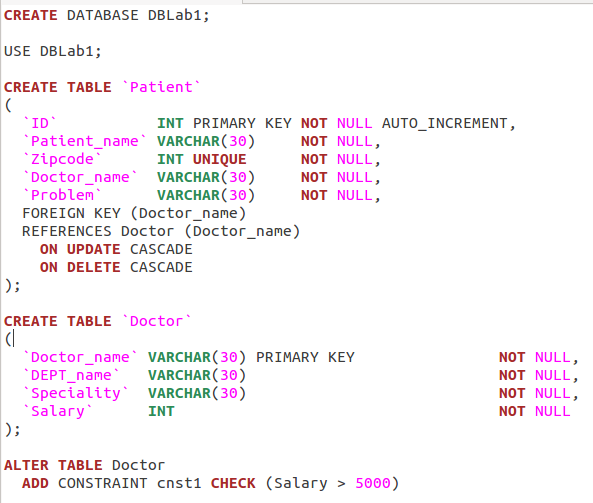
\includegraphics[scale=0.4]{figs/1.png}\
    \item
    ERD: 

		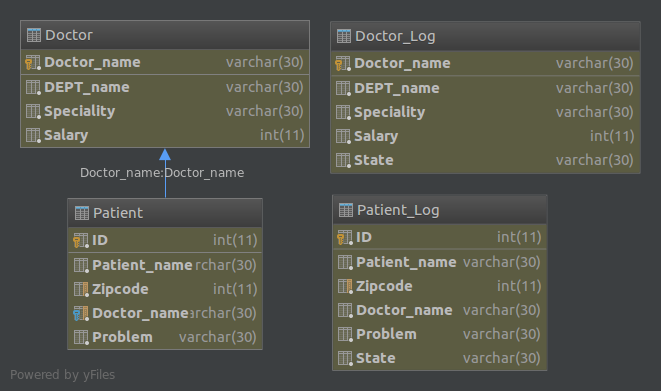
\includegraphics[scale=0.4]{figs/ERD.png}\
\end{itemize}
\section{Question 2:}
\begin{itemize}
    \item
    The procedure requested in question is written and code is shown below.
    
    	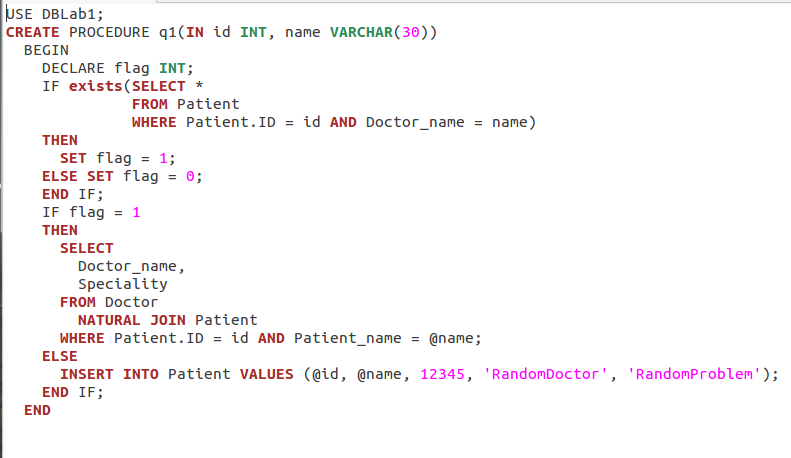
\includegraphics[scale=0.4]{figs/2.png}\
\end{itemize}
\section{Question 3:}
A function always returns a value but a procedure may return one or more value or may not return any value at all. The second difference is stored procedure returns always integer value by default zero. Whereas function returns type could be scalar or table or table values. Stored procedure is precompiled execution plan where as functions are not. Stored procedure has the security and reduces the network traffic and also we can call stored procedure in any no. of applications at a time. A Function can be used in the SQL Queries while a procedure cannot be used in SQL queries .that cause a major difference b/w function and procedures.
\begin{itemize}
    \item
    The function requested in question is written and code is shown below.
    
    	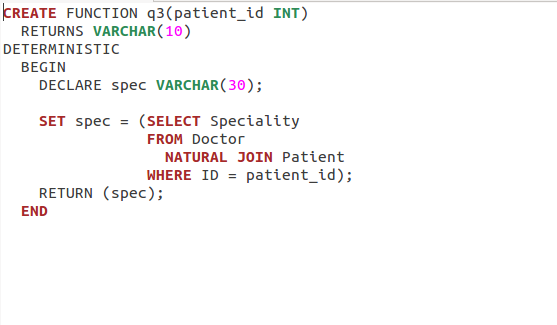
\includegraphics[scale=0.4]{figs/3.png}\
\end{itemize}
\section{Question 4:}
\begin{itemize}
    \item
    For this purpose, we need to add two more tables, so that we can insert logged data to them.
    
    	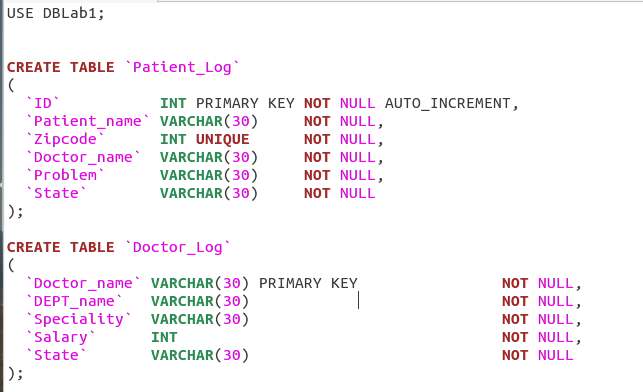
\includegraphics[scale=0.4]{figs/4_1.png}\
    \item
    Then triggers were created by code shown below.
    
		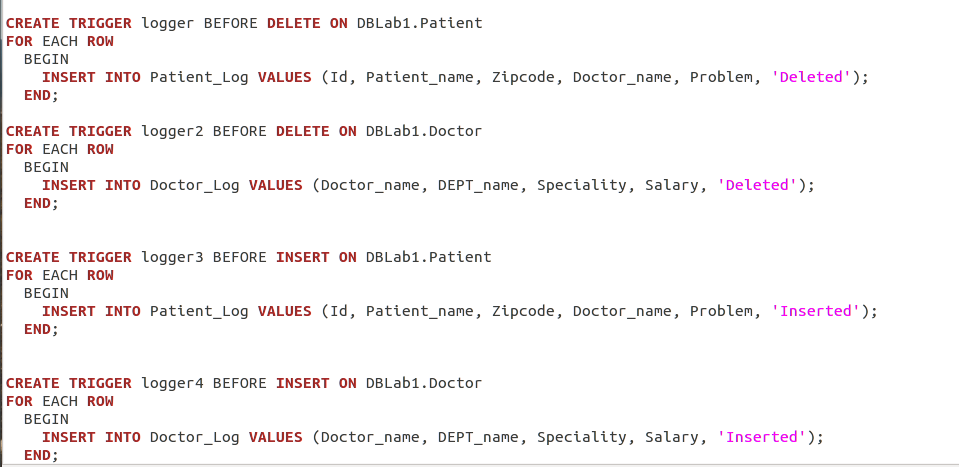
\includegraphics[scale=0.4]{figs/4_2.png}\
\end{itemize}
\end{document}